Dieser Abschnitt befasst sich mit der Verifizierung der Simulation. Dazu werden unterschiedliche Parameter der Simulation geändert und die Ergebnisse miteinander verglichen.\\
In einem ersten Schritt wird das Verhalten der Simulation bei standard Bedingungen angeschaut. Die standard Bedingungen werden hier aufgeführt:

\begin{tabbing}
\hspace{120mm}			\=  \hspace{10mm} \=	\\
Schlauchlänge			\> $10$m		\\
Schlauchdurchmesser		\> $5$cm		\\
Temperatur			\> $8^{\circ}$C		\\
Art der Flüssigkeit		\> Wasser	\> 		\\
\end{tabbing}

%%%%%%%%%%%%%%%%%%%%%%%%%%%%%%%%%%%%%%%%%%%%%%%%%%%%%%%%%%%%%%%%%%%%%%%%%%%%%
\begin{figure}[htb]
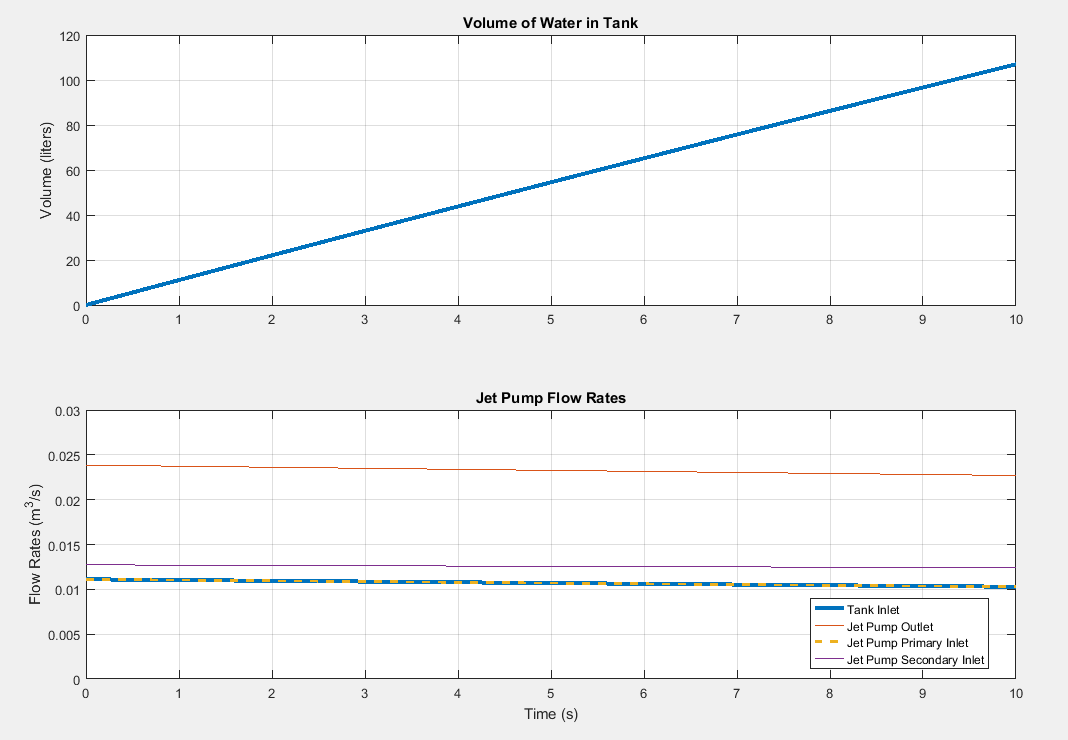
\includegraphics[width=\textwidth]{tank_10m_w.png}
\caption{Simulation mit standart Parameter}
\label{fig:Simulation mit standard Parameter}
\end{figure}
%%%%%%%%%%%%%%%%%%%%%%%%%%%%%%%%%%%%%%%%%%%%%%%%%%%%%%%%%%%%%%%%%%%%%%%%%%%%%

In der Abbildung \ref{fig:Simulation mit standard Parameter} ist zu sehen wie sich der Tank linear mit $10.864 l/s$ füllt. Der untere Teil der Abbildung zeigt den primären und sekundären Einlass in die Strahlpumpe und deren Auslass. Da der Sollwert für die Zentrifugalpumpe konstant ist verändern sich diese Werte nicht.\\
\\
Nun wird der Reihe nach an unterschiedlichen Parametern geschraubt. In einem ersten Schritt, wird das Verhalten der Simulation bei einer Verlängerung des Schlauches auf 100m angeschaut. Da sich dadurch der Widerstand des Schlauches erhöht wird ein kleinerer Durchfluss in den Tank erwartet. Tatsächlich liegt der Durchfluss nun bei $8 l/s$ (gem. Abb \ref{fig:Simulation mit veränderten Parametern}).
\clearpage

%%%%%%%%%%%%%%%%%%%%%%%%%%%%%%%%%%%%%%%%%%%%%%%%%%%%%%%%%%%%%%%%%%%%%%%%%%%%
\begin{figure}[htb]
    \subfigure[Simulation mit einem Schlauch von 100m]{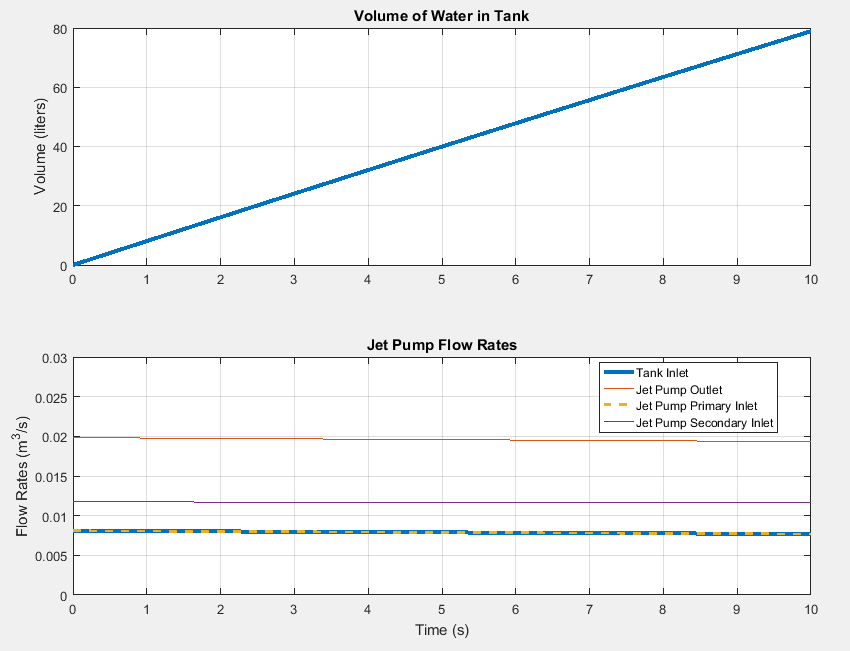
\includegraphics[width=0.49\textwidth, height=5cm]{tank_100m_w.png}}
    \subfigure[Simulation mit doppeltem Durchmesser]{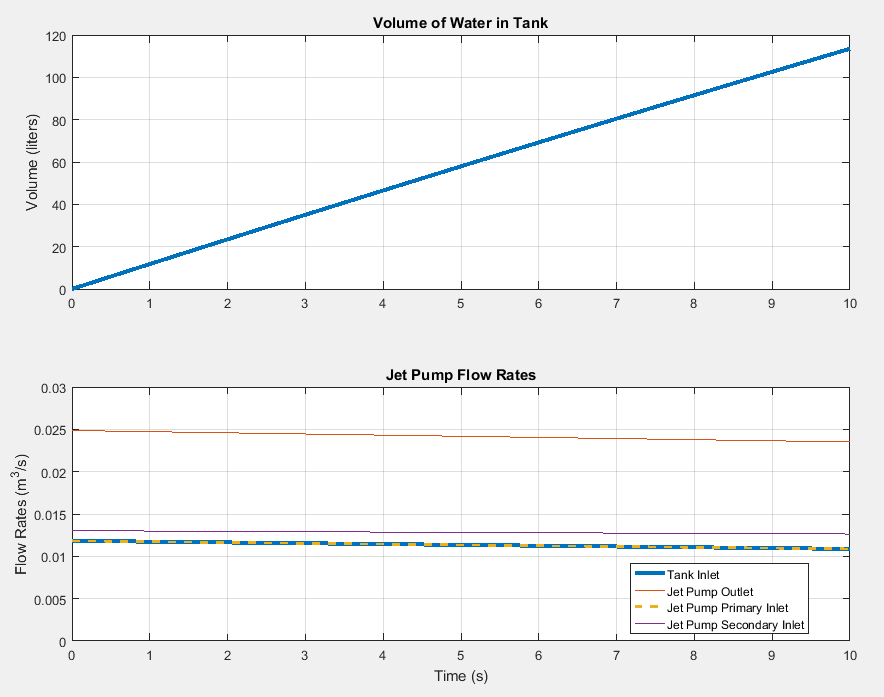
\includegraphics[width=0.49\textwidth, height=5cm]{tank_10m_10cm.png}}
\caption{Simulation mit veränderten Parametern}
\label{fig:Simulation mit veränderten Parametern}
\end{figure}
%%%%%%%%%%%%%%%%%%%%%%%%%%%%%%%%%%%%%%%%%%%%%%%%%%%%%%%%%%%%%%%%%%%%%%%%%%%%%

Als nächstes wird der Durchmesser des Schlauches auf das Doppelte erhöt. Nun erwarten wir einen grösseren Durchfluss da sich der Wiederstand des Schlauches verringert. Dadurch wird der Durchfluss auf $11.56 l/s$ erhöht (gem. Abb \ref{fig:Simulation mit veränderten Parametern}).\\
\\
In einem weiteren Versuch wird anstelle von Wasser Öl gepumpt. Genau genommen wird nun OIL-50W verwendet. Von Öl wird eine trägere Viskosität erwartet was dazu führen muss, dass sich eine kleinere Menge in das Schwimmbad leiten lässt, auch wenn dies im Falle eines Schwimmbeckens wahrscheindlich nie zur Anwendung kommt. Die Simulation verhält sich wie erwünscht und es können nur $3.5 l/s$ in den Tank gefördert werden (gem. Abb \ref{fig:Simulation mit veränderten Parametern 2}).\\
\\
Der letzte Versuch dient dazu den Einfluss der Zentrifugalpumpe zu überprüfen. Dazu wird der Sollwert der Pumpe auf die Hälfte reduziert. Daher wird ein kleinerer Durchfluss erwartet. Die Simulation verhält sich wie erwünscht und der Durchfluss reduziert sich auf $4.568 l/s$.\\
Die Simultation hat sich in jedem Punkt exakt so verhalten wie es von uns erwartet wurde. Dadurch lässt sich sagen, dass um die Füllmenge eines Schwimmbades zu simulieren, durchaus auf diese Simulation zurückgegriffen werden kann (gem. Abb \ref{fig:Simulation mit veränderten Parametern 2}).

%%%%%%%%%%%%%%%%%%%%%%%%%%%%%%%%%%%%%%%%%%%%%%%%%%%%%%%%%%%%%%%%%%%%%%%%%%%%
\begin{figure}[htb]
    \subfigure[Simulation mit Öl anstelle von Wasser]{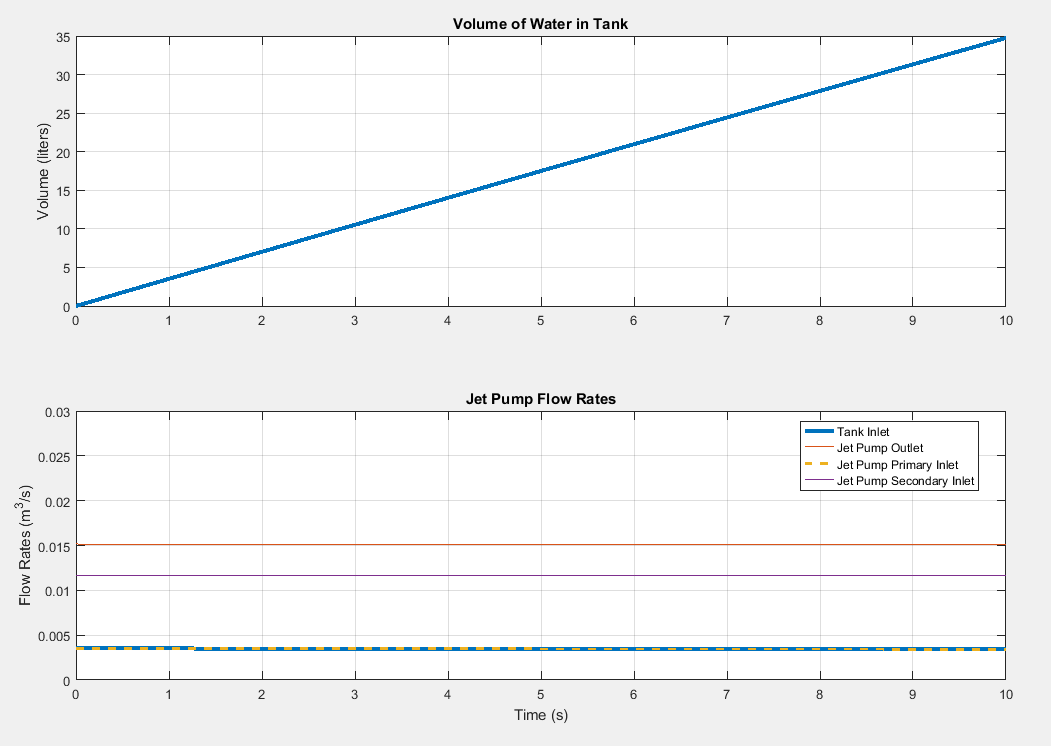
\includegraphics[width=0.49\textwidth, height=5cm]{tank_10m_o_50.png}}
    \subfigure[Simulation mit doppeltem Durchfluss]{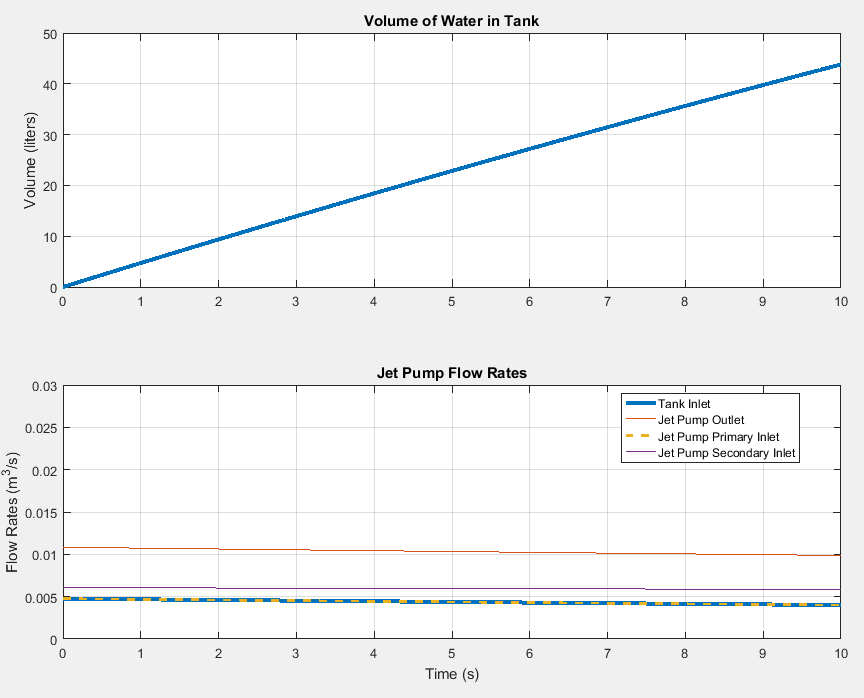
\includegraphics[width=0.49\textwidth, height=5cm]{tank_10m_2speed.png}}
\caption{Simulation mit veränderten Parametern}
\label{fig:Simulation mit veränderten Parametern 2}
\end{figure}
%%%%%%%%%%%%%%%%%%%%%%%%%%%%%%%%%%%%%%%%%%%%%%%%%%%%%%%%%%%%%%%%%%%%%%%%%%%%%


